\documentclass[UKenglish]{beamer}

\usepackage[utf8]{inputenx} % For æ, ø, å
\usepackage{csquotes}       % Quotation marks
\usepackage{microtype}      % Improved typography
\usepackage{amssymb}        % Mathematical symbols
\usepackage{mathtools}      % Mathematical symbols
\usepackage[absolute, overlay]{textpos} % Arbitrary placement
\setlength{\TPHorizModule}{\paperwidth} % Textpos units
\setlength{\TPVertModule}{\paperheight} % Textpos units
\usepackage{tikz}
\usetikzlibrary{overlay-beamer-styles}  % Overlay effects for TikZ

\AtBeginSection{\frame{\sectionpage}}
\AtBeginSubsection{\frame{\subsectionpage}}

\usepackage{hyperref}
\usepackage{svg}
%\usefonttheme{serif}

\usepackage{color, soul, xcolor} % Colored text and highlighting, respectively
\usepackage{tikz-cd} % For commutative diagrams
\usepackage{tikz-3dplot}
\usetikzlibrary{angles}
\RequirePackage{pgfplots}
\usepackage{mathtools}
\usepackage{answers}
\usepackage{setspace}
\usepackage{graphicx}
\usepackage{enumerate}
\usepackage{multicol}
\usepackage{mathrsfs}
\usepackage{amsmath,amsthm,amssymb}
\usepackage{marvosym,wasysym} %fucking smileys
\usepackage{float}
\usepackage{morefloats}
\usepackage{pgf,tikz}
\pgfplotsset{compat=1.15}
\usepackage{mathrsfs}
\usetikzlibrary{arrows}
\usepackage{subcaption}
\usepackage[most]{tcolorbox}
\tcbuselibrary{theorems}
\usepackage{fancyvrb}
\usepackage{longtable,booktabs}
\usepackage{stackrel}
\usepackage{animate}
\usepackage[percent]{overpic}
\definecolor{lighter_csu_green}{RGB}{60,133,77}
\newcommand\boldgreen[1]{\textcolor{lighter_csu_green}{\emph{\textbf{#1}}}}
\usepackage{MnSymbol}

%Commands
\newcommand{\R}{\mathbb{R}}
\newcommand{\opens}{\mathcal{O}}

%border matrix
\makeatletter
\newif\if@borderstar
\def\bordermatrix{\@ifnextchar*{%
\@borderstartrue\@bordermatrix@i}{\@borderstarfalse\@bordermatrix@i*}%
}
\def\@bordermatrix@i*{\@ifnextchar[{\@bordermatrix@ii}{\@bordermatrix@ii[()]}}
\def\@bordermatrix@ii[#1]#2{%
\begingroup
\m@th\@tempdima8.75\p@\setbox\z@\vbox{%
\def\cr{\crcr\noalign{\kern 2\p@\global\let\cr\endline }}%
\ialign {$##$\hfil\kern 2\p@\kern\@tempdima & \thinspace %
\hfil $##$\hfil && \quad\hfil $##$\hfil\crcr\omit\strut %
\hfil\crcr\noalign{\kern -\baselineskip}#2\crcr\omit %
\strut\cr}}%
\setbox\tw@\vbox{\unvcopy\z@\global\setbox\@ne\lastbox}%
\setbox\tw@\hbox{\unhbox\@ne\unskip\global\setbox\@ne\lastbox}%
\setbox\tw@\hbox{%
$\kern\wd\@ne\kern -\@tempdima\left\@firstoftwo#1%
\if@borderstar\kern2pt\else\kern -\wd\@ne\fi%
\global\setbox\@ne\vbox{\box\@ne\if@borderstar\else\kern 2\p@\fi}%
\vcenter{\if@borderstar\else\kern -\ht\@ne\fi%
\unvbox\z@\kern-\if@borderstar2\fi\baselineskip}%
\if@borderstar\kern-2\@tempdima\kern2\p@\else\,\fi\right\@secondoftwo#1 $%
}\null \;\vbox{\kern\ht\@ne\box\tw@}%
\endgroup
}
\makeatother

\usetheme{UiB}

%For easier reading
\setbeamersize{text margin left=40pt,text margin right=40pt}
\renewcommand{\baselinestretch}{1.3}


%% FONT STUFF
\usepackage{amsmath}
\usepackage{amsfonts}
\usefonttheme[onlymath]{serif}


\author{Colin Roberts}
\setbeamercolor{title}{fg=white} 
\title{Riemannian Geometry}
\setbeamercolor{subtitle}{fg=white} 
\subtitle{for Dummies}



\begin{document}


\section{Introduction}

\begin{frame}{}
	\vfill
	\large{Riemannian geometry} is the study of a \boldgreen{smooth manifold} $M$ along with a \boldgreen{Riemannian metric} $g$. 
	\vfill
\end{frame}

\begin{frame}{}
	\vfill
	The point of Riemmannian geometry is to generalize the differentiable and metric structure of $\R^n$.
	\vfill
\end{frame}

\begin{frame}{}
	\vfill
	We think of living on the manifold. We refer to this as \boldgreen{intrinsic}.
	\vfill
\end{frame}

\begin{frame}{}
	\vfill
	We generalize to spaces that have interesting topology and geometry.
	\vfill
\end{frame}

\begin{frame}{}
	\vfill
	This will require us to rethink some notions we found ``easy" in $\R^n$.
	\vfill
\end{frame}

\begin{frame}{}
	\vfill
	But we will gain a very general framework for working with differentiable objects.
	\vfill
\end{frame}

\section{Motivation}

\begin{frame}{}
	\vfill
	Why study this in the first place?
	\vfill
\end{frame}

\begin{frame}{}
	\vfill
	Example: Partial differential equations (PDEs) on spaces that are not flat.
	\pause
	\begin{itemize}
		\item Fluid flow on Earth
		\pause
		\item Electrical Impedence Tomography (EIT)
		\pause
		\item General relativity
	\end{itemize}
	\vfill
\end{frame}

\begin{frame}{}
	\vfill
	Example: Optimization in interesting spaces.
	\pause
	\begin{itemize}
		\item Matrix (symmetry) groups
		\pause
		\item Grassmannians, Flags
		\pause
		\item Curved spacetime
	\end{itemize}
	\vfill
\end{frame}

\begin{frame}{}
	\vfill
	Example: Rephrasing classical problems.
	\pause
	\begin{itemize}
		\item EIT
		\pause
		\item Polymer growth
		\pause
		\item Electrodynamics
	\end{itemize}
	\vfill
\end{frame}

\section{Preliminaries}


\subsection{Smooth Manifolds}

\begin{frame}{}
\vfill
\textbf{\underline{Our To-Do List:}}
\begin{itemize}
	\item Start with a topological space $M$
	\pause
	\item Look at open sets $U$ that cover $M$
	\pause
	\item Construct local coordinates $\varphi$
	\pause
	\item Show coordinate transition functions are smooth
\end{itemize}
\vfill
\end{frame}

\begin{frame}{}
	\vfill
	Working example: 2-sphere
	\[
		S^2 \coloneqq \{(x,y,z) \in \R^3 ~\vert~ x^2+y^2+z^2=1\}.
	\]
	\vfill
\end{frame}

\begin{frame}{}
\vfill
\begin{figure}[H]
	\centering
	\def\svgwidth{0.75\columnwidth}
	\input{sphere.pdf_tex}
\end{figure}\vfill
\end{frame}

\begin{frame}{}
	\vfill
	Take open sets in $\R^m$
	\[
	\mathcal{O}_\alpha \qquad \mathcal{O}_\beta
	\]
	\pause
	and maps
	\[
	\varphi_\alpha \colon \mathcal{O}_\alpha \to U_\alpha \subset M \qquad 	\varphi_\beta \colon \mathcal{O}_\beta \to U_\beta \subset M.
	\]
	\pause
	These are our \boldgreen{local coordinates}.
	\vfill
\end{frame}

\begin{frame}{}
\vfill
\begin{figure}[H]
	\centering
	\def\svgwidth{.75\columnwidth}
	\input{sphere_charts.pdf_tex}
\end{figure}
\vfill
\end{frame}

\begin{frame}{}
	\vfill
	Our local coordinates must work together on overlaps
	\[
	U_\alpha \cap U_\beta.
	\]
	\pause
	We check the \boldgreen{transition function} 
	\[
	\phi_{\alpha\beta} = \varphi_\alpha^{-1} \circ \varphi_\beta
	\]
	is smooth and invertible as a function on $\R^m$.
	\vfill
\end{frame}


\begin{frame}{}
\vfill
\begin{figure}[H]
	\centering
	\def\svgwidth{\columnwidth}
	\input{sphere_charts_maps.pdf_tex}
\end{figure}
\vfill
\end{frame}

\subsection{Vector Fields}

\begin{frame}{}
	\vfill
	Vector fields on $\R^m$ are functions $\vec{f}\colon \R^m \to \R^m$.
	\begin{figure}
	   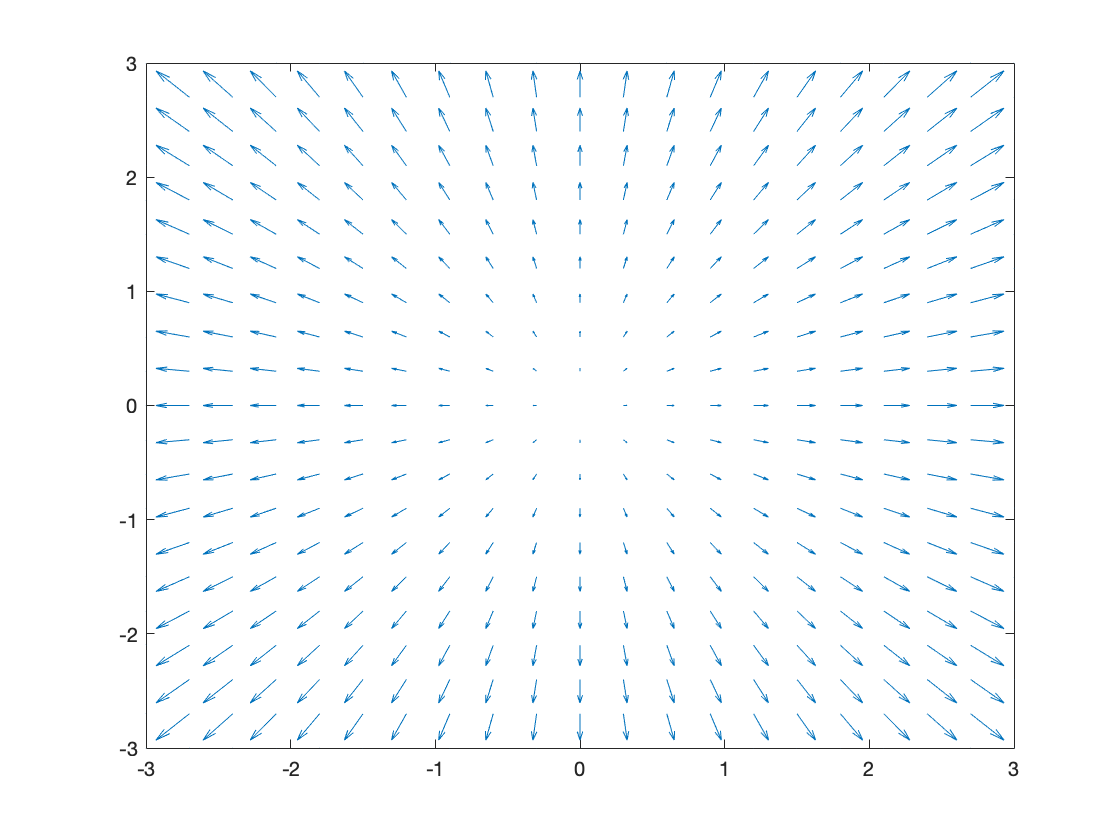
\includegraphics[width=0.49\textwidth]{div_field.png}
	   \hfill
	   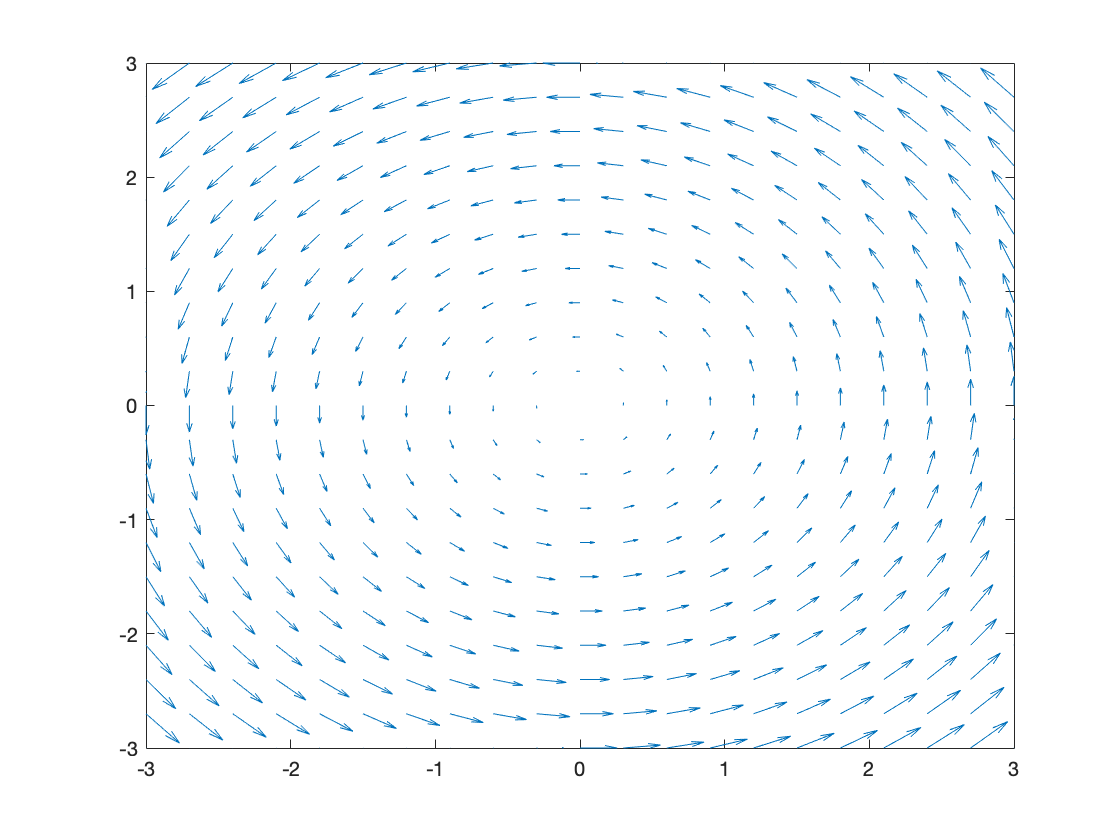
\includegraphics[width=0.49\textwidth]{rot_field.png}
	\end{figure}
	\pause
	Intrinsic vector fields on manifolds carry geometric information.
	\vfill
\end{frame}

\begin{frame}{}
\vfill
\textbf{\underline{Our To-Do List:}}
\begin{itemize}
	\item Construct the \boldgreen{tangent space} $T_pM$
	\pause
	\item Glue together tangent spaces to form the \boldgreen{tangent bundle} $TM$
	\pause
	\item Properly define vector fields $X$ as \boldgreen{sections} of the tangent bundle
\end{itemize}
\vfill
\end{frame}

\begin{frame}{}
	\vfill
	\begin{itemize}
		\item Start with a curve $\gamma (-1,1) \to M$ with $\gamma(0)=p$
		\pause
		\item Find the velocity vector $\dot{\gamma}=\left.\frac{d\gamma}{dt}\right\vert_{t=0}$
		\pause
		\item This defines a tangent vector at $p$
		\pause
		\item All possible tangent vectors form the tangent space $T_pM$.
	\end{itemize}
\end{frame}

\begin{frame}{}
\vfill
\begin{figure}[H]
	\centering
	\def\svgwidth{0.75\columnwidth}
	\input{sphere_curve.pdf_tex}
\end{figure}
\vfill
\end{frame}

\begin{frame}{}
\vfill
\begin{figure}[H]
	\centering
	\def\svgwidth{0.75\columnwidth}
	\input{sphere_curve_tangent.pdf_tex}
\end{figure}
\vfill
\end{frame}

\begin{frame}{}
	\vfill
	We need to understand how tangent vectors on $M$ relate to vectors in our local coordinates $\varphi$.
	\begin{itemize}
		\item The differential $d\varphi$ is a map of tangent vectors
		\pause
		\item If $\varphi(x)=p$, then $d\varphi(x) \colon T_x\R^m \to T_pM$
	\end{itemize}
	\vfill
\end{frame}

\begin{frame}{}
\vfill
\begin{figure}[H]
	\centering
	\def\svgwidth{\columnwidth}
	\input{pushforward.pdf_tex}
\end{figure}
\vfill
\end{frame}

\begin{frame}{}
	\vfill
	\begin{itemize}
		\item We need to understand how different tangent spaces relate
		\pause
		\item Properly gluing tangent spaces $T_pM$ to the manifold $M$ allows us to build a larger manifold $TM$.
		\pause
		\item This allows us to see how tangent vectors move around the whole manifold.
	\end{itemize}
	\vfill
\end{frame}

\begin{frame}{}
	\vfill
	We briefly drop a dimension to the 1-sphere
	\[
	S^1 \coloneqq \{ (x,y)\in \R^2 ~\vert~ x^2+y^2 = 1\}.
	\]
	\vfill
\end{frame}

\begin{frame}{}
\vfill
\begin{figure}[H]
	\centering
	\def\svgwidth{.75\columnwidth}
	\input{tangent_spaces.pdf_tex}
\end{figure}
\vfill
\end{frame}

\begin{frame}{}
\vfill
\begin{figure}[H]
	\centering
	\def\svgwidth{\columnwidth}
	\input{tangent_bundle.pdf_tex}
\end{figure}
\vfill
\end{frame}

\begin{frame}{}
	\vfill
	\begin{itemize}
		\item Points in $TM$ are $(p,v)$ with $p\in M$ and $v\in T_pM$
		\pause
		\item So, a function $X \colon M \to TM$ selects a tangent vector at every point
		\pause
		\item For example, $X_p = v \in T_pM$
		\pause
		\item We have the projection $\pi \colon TM \to M$ by $\pi(p,v)=p$
		\pause
		\item $X$ is a \boldgreen{section} if $\pi \circ X = \mathrm{Id_M}$ (vertical line test)
	\end{itemize}
\end{frame}

\begin{frame}{}
\vfill
\begin{figure}[H]
	\centering
	\def\svgwidth{\columnwidth}
	\input{section.pdf_tex}
\end{figure}
\vfill
\end{frame}

\begin{frame}{}
	\vfill
	\centering
	Back to the 2-sphere.
	\vfill
\end{frame}

\begin{frame}{}
\vfill
\begin{figure}[H]
	\centering
	\def\svgwidth{.75\columnwidth}
	\input{sphere_vector_field.pdf_tex}
\end{figure}
\vfill
\end{frame}

\subsection{Specific Coordinates}

\begin{frame}{}
	\vfill
	We should work with specific coordinates on $S^2$.
	\vfill
\end{frame}

\begin{frame}{}
\vfill
\begin{figure}[H]
	\centering
	\def\svgwidth{\columnwidth}
	\input{spherical_coordinates.pdf_tex}
\end{figure}
\vfill
\end{frame}

\begin{frame}{}
\vfill
\begin{figure}[H]
	\centering
	\def\svgwidth{\columnwidth}
	\input{spherical_coordinates_tangent_vectors.pdf_tex}
\end{figure}
\vfill
\end{frame}

\begin{frame}{}
	\vfill
	\begin{itemize}
		\item We can take a vector field in $\R^m$ and push it forward onto $M$
		\pause
		\item We extend the differential $d\varphi(x) \colon T_xM \to T_pM$ to a map on bundles
		\pause
		\item This bundle map $\varphi_* \colon T\R^m \to TM$ is the \boldgreen{pushforward}
	\end{itemize}
\end{frame}

\begin{frame}{}
\vfill
\begin{figure}[H]
	\centering
	\def\svgwidth{\columnwidth}
	\input{push_forward.pdf_tex}
\end{figure}
\vfill
\end{frame}

\section{Riemannian Geometry}

\begin{frame}{}
\vfill
\textbf{\underline{Our To-Do List:}}
\begin{itemize}
	\item Build an inner product on the tangent space $T_pM$;
	\pause
	\item Have the inner product vary smoothly as we vary the point $p$;
	\pause
	\item Define this as our Riemannian metric tensor field $g$;
	\pause
	\item Extract geometrical and analytical qualities of the underlying manifold $M$.
\end{itemize}
\vfill
\end{frame}


\subsection{Riemannian Metric}

\begin{frame}{}
	\vfill
	We use the differential and dot product to form a matrix at each point
	\[
	g_{ij}(x) = d\varphi(x)e_i \cdot d\varphi(x)e_j.
	\]
	\pause
	This matrix is the \boldgreen{Riemannian metric}.
	\vfill
\end{frame}

\begin{frame}{}
	\vfill
	Riemannian metric provides an inner product for tangent vectors on $M$. Thus, we know
	\begin{itemize}
		\item how lengths are distorted;
		\item how volume is distorted.
	\end{itemize}
	This allows us to integrate or differentiate in our coordinates but think of it as intrinsic to the manifold.
	\vfill
\end{frame}

\begin{frame}{}
	\vfill
	\begin{itemize}
		\item The Riemannian metric gives us a distance function $d(p,q)$ on $M$
		\pause
		\item Compute this by finding the length of the shortest curve 
		\[
		\gamma\colon [0,1]\to M \qquad \gamma(0)=p,~\gamma(1)=q
		\]
		\pause
		We need to solve
		\[
		\inf_{\gamma} \ell(\gamma) \coloneqq \int_0^1 \sqrt{g(\dot{\gamma},\dot{\gamma})}dt
		\]
	\end{itemize}
\end{frame}

\begin{frame}{}
	\vfill
	\begin{itemize}
		\item Reminder: in $\R^m$, the speed of a curve is $\sqrt{\dot{\gamma},\dot{\gamma}}$
		\pause
		\item $g(\dot{\gamma},\dot{\gamma})$ is the speed on $M$
		\pause
		\item We put $g(\dot{\gamma},\dot{\gamma})$ to mean $\sum_{i,j=1}^m g_{ij} \dot{\gamma}_i \dot{\gamma}_j$.
	\end{itemize}
	\vfill
\end{frame} 

\begin{frame}{}
\vfill
\begin{figure}[H]
	\centering
	\def\svgwidth{.75\columnwidth}
	\input{curves.pdf_tex}
\end{figure}
\end{frame}

\begin{frame}{}
	\vfill
	Solving this optimization problem yields the \boldgreen{geodesic equation}
	\[
		\ddot{x}^l +\dot{x}^j\dot{x}^k \Gamma_{jk}^l = 0
	\]
	where $\Gamma_{jk}^l$ are the \boldgreen{Christoffel symbols} which are formed by derivatives of the metric.
	\vfill
\end{frame}

\begin{frame}{}
	\vfill
	This defines an intrinsic derivative $\nabla$ called the \boldgreen{Levi-Civita connection}
	\vfill
\end{frame}

\begin{frame}{}
	\vfill
	\begin{itemize}
		\item Since we know how vectors are transformed, combining those describes transformed volumes.
		\pause
		\item The determinant gives us area information.
		\pause
		\item Then $\sqrt{|\det(g(x))|}$ gives us the volume on $M$
	\end{itemize}
	\vfill
\end{frame}

\begin{frame}{}
	\vfill
	In spherical coordinates, $\sqrt{|\det(g)|} = \sin \varphi$ which gives us the integrand
	\[
		\sin\varphi d\varphi d\theta.
	\]
	\vfill
\end{frame}

\begin{frame}{}
\vfill
\begin{figure}[H]
	\hspace*{-2cm}
	\def\svgwidth{1.2\columnwidth}
	\input{area.pdf_tex}
\end{figure}
\end{frame}

\section{Conclusions}

\begin{frame}{}
	\vfill
	\begin{itemize}
		\item We constructed a smooth manifold $M$
		\pause
		\item We generalized vector fields $X$ to $M$
		\pause
		\item We created an inner product $g$ on $M$ to measure these fields
		\pause
		\item No measurement depends on the choice of coordinates
	\end{itemize}
	\vfill
\end{frame}

\begin{frame}{}
	\vfill
	\begin{itemize}
		\item $g$ allows us to measure vectors and understand the geometry of $M$ in coordinates $\varphi$
		\pause
		\item Hence, we can define lengths and volumes
		\pause
		\item Thus, we can integrate
	\end{itemize}
	\vfill
\end{frame}

\begin{frame}{}
	\vfill
	\begin{itemize}
		\item $g$ induces a derivative $\nabla$
		\pause
		\item $g$ induces a Laplacian $\Delta$
		\pause
		\item $g$ provides an intrinsic length function on $M$
	\end{itemize}
	\vfill
\end{frame}

\begin{frame}{}
	\vfill
	This is just the beginning!
	\vfill
\end{frame}


\end{document}



%%% MAYBE USEFUL
%\begin{frame}{}
%	\vfill
%	A \boldgreen{topological space} $M$ is a set of points with a collection of subsets $\opens$ that we define to be open. These sets satisfy \pause
%	\begin{itemize}
%		\item $\emptyset,M \in \opens$;
%		\pause
%		\item Arbitrary unions of open sets are open;
%		\pause
%		\item Finite intersections of open sets are open.
%	\end{itemize}
%	\vfill
%\end{frame}
%
%\begin{frame}{}
%	\vfill
%Just do diffeomorphisms and forget this
%	\begin{itemize}
%		\item A \boldgreen{homeomorphism} is a continuous bijection $f\colon M \to N$ with continuous inverse $f^{-1}$.  
%		\pause
%		\item We say $M$ and $N$ are homeomorphic.
%	\end{itemize}
%	\vfill	
%\end{frame}
%
%\begin{frame}{}	
%	ignore boundary 
%	\vfill
%	A \boldgreen{manifold} (with boundary) is a space that locally looks like $\R^n$ (or $\R^{n^+}$). 
%	\pause	
%	\[
%	\downarrow
%	\]
%	A \boldgreen{manifold} $M$ (with boundary) is a topological space such that each open set in $\opens$ is homeomorphic to $\R^n$ (or $\R^{n^+}$).
%	\vfill
%\end{frame}
%
%\begin{frame}{}
%	\vfill
%	
%\end{frame}
%
%\begin{frame}{}
%	
%\end{frame}
%
%\begin{frame}{Manifolds}
%	\begin{figure}[H]
%    \centering
%    \begin{overpic}[width=0.8\textwidth]{Figures/coordinate_charts_manifold.png}
%    \put (39,61) {\Large$U_\alpha$}
%    \put (70,57) {\Large$U_\beta$}
%    \put (12,65) {\LARGE$M$}
%    \put (20,35) {\Large$\varphi_\alpha$}
%    \put (73,30) {\Large$\varphi_\beta$}
%    \put (22,3) {\Large$\R^m$}
%    \put (60,3) {\Large$\R^m$}
%    \put (38,32) {\Large$\varphi_{\alpha \beta}$}
%    \put (38,18) {\Large$\varphi_{\beta \alpha}$}
%    \end{overpic}
%\end{figure}
%\end{frame}